\subsection{Grundlagen}
\paragraph{Neue Anforderungen an Robotersysteme}
\begin{itemize}
\item In der \textbf{Produktion}: Klein- \& Kleinstserienfertigung, Unikatfertigung (z.B. Prototyp)\\
$\rightarrow$ Produkte mit: vielen Ausstattungsvarianten und hoher Rekonfigurierbarkeit\\
$\rightarrow$ Flexible Fertigung
\item Im \textbf{Servicebereich}: \\
$\rightarrow$ Handel:  Kommissionierung und Palettierung von Waren, Bestücken von Regalen\\
$\rightarrow$ Pflege: Unterstützung von Rehabilitationsmaßnahmen durch Roboter, Rollstuhl mit Manipulationshilfe\\
$\rightarrow$ Handwerk: Handhabungen in Schreinereien und Schlossereien
\item In der \textbf{humanoiden Servicerobotik}: Manipulation beliebiger Objekte, selbstständiges Lösen komplexer Aufgaben, Einsatz im menschlichen Umfeld\\
$\rightarrow$ komplexe Umgebung und sehr viele Freiheitsgrade\\
$\rightarrow$ Wie Handlungswissen erzeugen?
\end{itemize}

\subsubsection*{Grundidee der interaktiven Programmierung} %5.1.1.
\begin{itemize}
\item[1.]Mensch ist Domänenexperte (Manipulation)
\item[2.]Explizite Demonstrationen der Manipulationsaufgabe
\item[3.]Sensorielle Erfassung der Demonstrationen
\item[4.]Erzeugung der internen Repräsentation des Roboterprogramms
\item[5.]Abbildung auf das Robotersystem
\item[6.]Ausführung
\end{itemize}

\subsubsection*{Anforderungen an interaktive Programmierung}
\begin{itemize}
\item[1.]Intuitive Interaktionsformen: einfache Bedienung des Systems
\item[2.]Transparenz der Prozesse im Programmiersystem: Umsetzung von Handlungen des Benutzers soll nachvollziehbar sein
\item[3.]Abgleich von Systemhypothesen mit der Benutzerintention: z.B. zur Korrektur falscher Systemhypothesen
\item[4.]Flexibilisierung und Optimierung von Programmen: erlernte Programme sollen in vielen Situationen anwendbar sein
\item[5.]Wiederverwendung von Teillösungen: Funktionsbausteine sollen in anderen Pogrammen wiederverwendbar sein
\end{itemize}

\subsubsection*{Randbedingungen}
Notwendig zur Erzeugung von leistungsfähigen, automatischen aber auch sicheren und komfortablen Roboterprogrammen
\begin{itemize}
\item[1.]Weitgehend automatisierte Programmgenerierung
\item[2.]Beschränkung der Benutzerinteraktion auf das Nötigste
\item[3.]Maximierung des Informationsgewinns und der Eindeutigkeit der Ergebnisse der Benutzerinteraktion für das System
\item[4.]Möglichst benutzerfreundliche Mensch-Maschine Interaktion: verständlich, transparent und flexibel, möglichst ähnlich zur zwischenmenschlichen Kommunikation
\end{itemize}

\subsection{PdV - Generelles Framework}
\begin{figure}[ht]\centering 
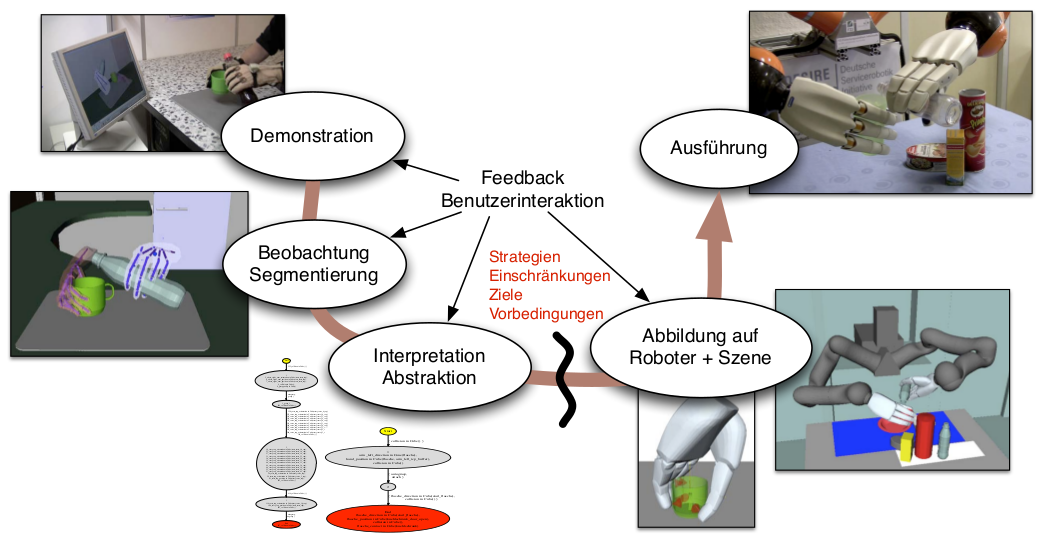
\includegraphics[width=0.6\linewidth]{figures/ch03_zyklus.png}
\caption{PdV-Zyklus}
\label{fig:ch03_zykl}
\end{figure}
Abbildung  \ref{fig:ch03_zykl} zeigt die Phasen von PdV.
\subsubsection*{Beobachtung}
Beobachtung der Benutzerinteraktion mittels externer und interner Sensorik (z.B. Kamerasysteme, Datenhandschuhe, Positionstracker).
\begin{itemize}
\ita mit den gewonnenen Sensordaten lassen sich dann Objekte klassifizieren, Trajektorien aufzeichnen und weitere Vorverarbeitungsschritte wie
Grifferkennung durchführen
\end{itemize}

\subsubsection*{Segmentierung}
Segmentierung in relevante Operationen oder Umweltzustände. 
\begin{itemize}
\item man benötigt hierfür die Trajektorien aus der Demonstration, eine Datenbasis mit den Sensordaten, einen Satz Aktionstypen (Griffe, Lageänderungen von Objekten), einen Satz
von Elementaroperationen und das Umweltmodell
\item durch eine geeignete Heuristik lässt sich damit die Segmentierung durchführen
\item eine zusätzlich Interaktion mit dem Benutzer (über verschiedene Kommunikationskanäle wie grafische Benutzerschnittstellen oder Sprache) hilfreich; 
Rückfragen helfen bei der Identifikation der in der Lösung involvierten Objekte und sparen damit unnötige Berechnungen aller Relationen zwischen allen Objekten
ein
\item Rauschfilterung
\end{itemize}
\subsubsection*{Interpretation/Abstraktion}
Abstraktion von der Demonstration um die Lösung der Aufgabe so allgemein wie möglich darzustellen.
\begin{itemize}
\ita Instanzen müssen falls möglich in Variablen umgewandelt werden; dabei muss sichergestellt werden, dass in der Ausführungsphase nur solche Variablen instantiiert
werden, die räumliche Vorbedingungen erfüllen. Es wird also für jeden \Gu generalisierten\Go Operator ein Satz von Vorbedingungen in Form von wichtigen Relationen
gespeichert. Generiert werden diese Vorbedingungen mit Hilfe von Hintergrundwissen und wiederum durch Rückfragen an den Benutzer. Man benötigt also eine deduktive
Komponente, die die generalisierten Operatoren in Makro-Operatoren gruppiert. Da Makro-Operatoren weitere Makro-Operatoren als Kinder beinhalten können, lässt
sich die gesamte Benutzervorführung auf verschiedenen Abstraktionsebenen darstellen. Durch die Generalisierung lässt sich die Lösung später auf ähnliche Problemklassen anwendbare Lösungsbeschreibungen abbilden. In dieser Phase lassen sich auch vom Demonstrator durchgeführte spontane und nicht zielorientierte Bewegungen ausfiltern.
\end{itemize}
\subsubsection*{Transfer/Abbildung auf Roboter \& Szene}
Transfer der internen Wissensrepräsentation auf das Zielsystem. Aus den zuvor gewonnenen semantischen Informationen lässt sich jetzt ein ausführbares Roboterprogramm generieren. Dafür müssen die Operationen auf die Operationen des Zielsystems abgebildet werden. Die Ausgabe dieser Phase ist eine Sequenz von Elementarbewegungen, die nur für das Zielsystem und das jeweilige Umweltmodell gültig sind. Diese kann direkt in das Simulationsmodul weitergeleitet werden.
\subsubsection*{Simulation}
Simulation des physikalischen Vorgangs zur Validierung der getroffenen Entscheidungen. In der Simulation wird die gelernte Aufgabe von einem virtuellen Modell des Roboters in einer virtuellen Umwelt an virtuellen Objekten ausgeführt. Anhand einer visuellen Ausgabe lässt sich vom Benutzer die korrekte Ausführung der Aufgabe überprüfen. 
\subsubsection*{Ausführung}
Ausführung auf dem Zielsystem. Die zuvor validierte Sequenz elementarer Roboterbewegungen wird an den Roboter-Controller weitergereicht. Wenn bei der Modellierung in der Simulationsphase keine Fehler gemacht wurden, ist es sehr wahrscheinlich, dass die Ausführung nicht fehlschlagen wird-

\subsection{Klassifikation von PdV-Verfahren}
\begin{figure}[ht]\centering 
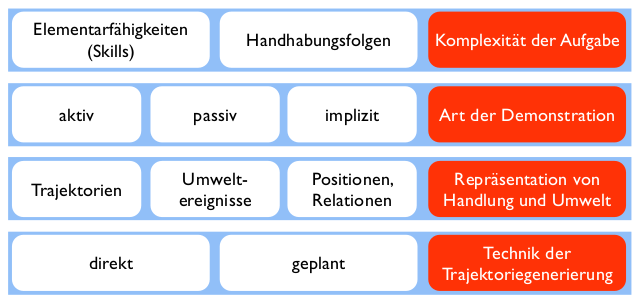
\includegraphics[width=0.6\linewidth]{figures/ch03_kriterien.png}
\caption{Klassifikationskriterien}
\label{fig:ch03_krit}
\end{figure}
Abbildung  \ref{fig:ch03_krit} zeigt die Klassifikationskriterien auf einen Blick.
\subsubsection*{Komplexität der Aufgabe}
Siehe Tabelle \ref{tab:aufgkomp}
\begin{table}[hbt]
\centering
\begin{tabular}{|p{8cm}|p{8cm}|}
\hline
Elementarfähigkeiten & Komplexe Aufgaben\\
\hline
Reflexe, Basisskills, einfache Bewegungen 
\vspace{-4mm}
\begin{itemize}
\setlength\itemsep{0em}
\item Lernen direkter Sensor-/Aktorzusammenhänge
\item Beispiele: Verwendung neuronaler Netze auf adaptive Regelkreise, Zustandsautomaten \footnote{Asada91, Koeppe95, Kaiser96, Ishikawa99, Bentivegna00, Calinon08, Pastor09}
\item[$\rightarrow$] Probleme: Explizite Beispiele, stark konfigurationsabhängig,
viele Trainingsbeispiele notwendig
\end{itemize}
 &
Task, Montageaufgaben
 \vspace{-4mm}
\begin{itemize}
\setlength\itemsep{0em}
\item Interpretation von Handlungsfolgen\footnote{Segre89, Inaba90, Kang94, Sagerer98, Aleotti06, Pardowitz07
Veeraraghavan08}
\ita Probleme: Breites Hintergrund-, Planungs- und Modellwissen,
Klärungsdialoge mit dem Benutzern
\end{itemize}\\
\hline
\end{tabular}
\caption{Kriterium 1 - Komplexität der Aufgabe}
\label{tab:aufgkomp}
\end{table}
\subsubsection*{Art der Demonstration}
Siehe Tabelle \ref{tab:demo}
\begin{table}[hbt]
\centering
\begin{tabular}{|p{5cm}|p{5cm}|p{5cm}|}
\hline
aktiv & passiv & implizit\\
\hline
Aktive Beispiele
\vspace{-4mm}
\begin{itemize}
\setlength\itemsep{0em}
\item Benutzer führt explizit vor
\item Beobachtung durch Sensorsystem (Datenhandschuh, Kameras)\footnote{Friedrich98, Ikeuchi99, Inoue/Kuniyoshi94, Zöllner06}
\ita Probleme: Aufwendige Sensorsysteme, Identifikation relevanter Aktionen und Ziele bzw. Zustände schwierig
\end{itemize}
 &
Passive Beispiele
 \vspace{-4mm}
\begin{itemize}
\setlength\itemsep{0em}
\item Roboter wird duch externen \Gu Master\Go
gesteuert, Signalaufzeichnung, Korrelation
zwischen Sensor- und Aktordaten\footnote{Kaiser96, Koeppe98, Billard07}
\ita Probleme: Gelerntes Wissen ist auf
konkretes Zielsystem festgelegt
\end{itemize} 
&
Implizite Beispiele
 \vspace{-4mm}
\begin{itemize}
\setlength\itemsep{0em}
\item Zielspezifikation durch Vorgabe graphischer Ikone\footnote{Takahashi/Ogata97,Sagerer98, Riepp97}
\ita Probleme: Dialog umfangreich, Anpassung an Zielsystem
\end{itemize}\\
\hline
\end{tabular}
\caption{Kriterium 2 - Art der Demonstration}
\label{tab:demo}
\end{table}

\subsubsection*{Repräsentation von Handlung und Umwelt}
Siehe Tabelle \ref{tab:rep}
\begin{table}[hbt]
\centering
\begin{tabular}{|p{5cm}|p{5cm}|p{5cm}|}
\hline
Trajektorien & Umweltereignisse & Positionen, Relationen\\
\hline
\vspace{-4mm}
\begin{itemize}
\setlength\itemsep{0em}
\ita Problem: keine wesentliche Generalisierung (1:1 Abbildung)
\end{itemize}
 &
Wirkungen und Reaktionen auf die Umgebung
 \vspace{-4mm}
\begin{itemize}
\setlength\itemsep{0em}
\ita Probleme: Identifikation von Kausalitäten und
Zustandsfolgen durch kognitive Operatoren
\end{itemize} 
&
Objektlagen, Relationen und Operatoren
 \vspace{-4mm}
\begin{itemize}
\setlength\itemsep{0em}
\ita Probleme: Beschränkung auf vorgegebenen
Operatorumfang
\end{itemize}\\
\hline
\end{tabular}
\caption{Kriterium 3 - Repräsentation von Handlung und Umwelt}
\label{tab:rep}
\end{table}
\subsubsection*{Technik der Trajektoriengenerierung}
Siehe Tabelle \ref{tab:trajtech}
\begin{table}[hbt]
\centering
\begin{tabular}{|p{8cm}|p{8cm}|}
\hline
geplant & direkt \\
\hline
Planung von Roboterbewegungen / Aktionen
\vspace{-4mm}
\begin{itemize}
\setlength\itemsep{0em}
\item Planung erforderlich zur Berücksichtigung der Unterschiede in
Demonstrations- und Ausführungsumgebung
\item Vollständige Nutzung der Leistungsfähigkeit des Robotersystems
\ita Probleme: Umwelt- und Planungswissen erforderlich,
intelligentes Planungssystem
\end{itemize}
 &
Direkte Abbildung
 \vspace{-4mm}
\begin{itemize}
\setlength\itemsep{0em}
\item Explizites oder gelerntes Transformationsmodell\footnote{Kang97, Kaneko97}
\ita Probleme: Zielsystem und Zielumgebung müssen korrespondieren
\end{itemize}\\
\hline
\end{tabular}
\caption{Kriterium 4 - Technik der Trajektoriengenerierung}
\label{tab:trajtech}
\end{table}

\subsection{Prozesskomponenten der interaktiven Programmierung}
\begin{figure}[ht]\centering 
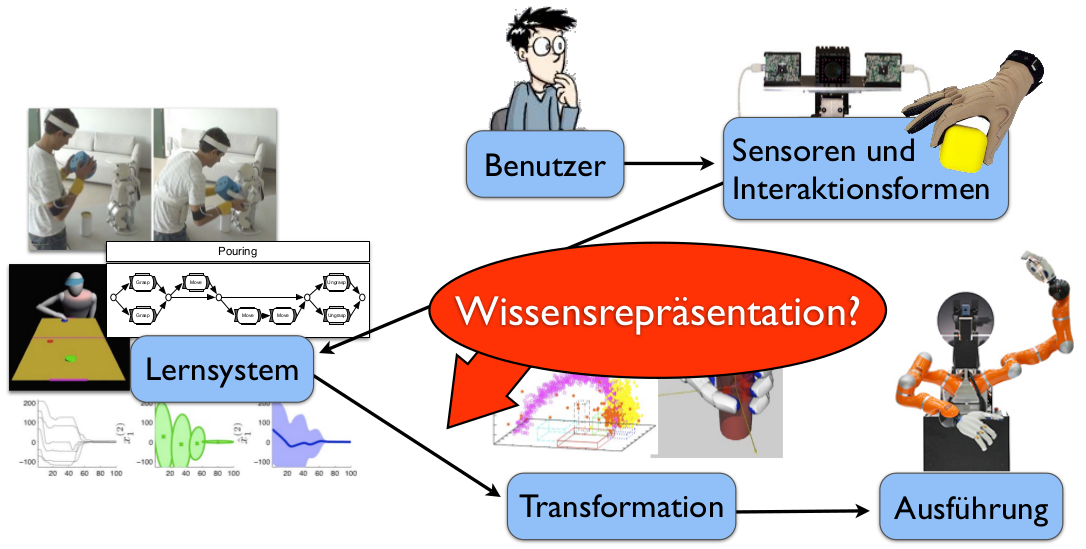
\includegraphics[width=0.6\linewidth]{figures/ch03_komponenten.png}
\caption{Interaktive Programmierung: Komponenten}
\label{fig:ch03_kom}
\end{figure}
Abbildung \ref{fig:ch03_kom} skizziert die an PdV beteiligten Komponenten:
\subsubsection*{Benutzer und Mensch-Maschine-Interaktionsformen}
Der Mensch, welcher die interaktive Programmierung vornimmt, kann multimodal mit dem Programmiersystem interagieren:
\begin{itemize}
\item \textbf{Physische Demonstration:}
Hierbei vollzieht der Benutzer die Manipulationsaufgabe mit realen Objekten und wird dabei
vom Programmiersystem durch Sensoren erfasst und seine Handlungen aufgezeichnet. 
Dies ist die natürlichste Art der Demonstration: Objekte können direkt mit den Händen 
oder mittels spezieller Vorführgeräte (z.B. Laserstift, 6D-Kugel) manipuliert werden. 
In jedem Fall ein großes Maß an Konzentration auf Seiten des Benutzers gefordert\\
Nachteile: 
\begin{itemize}
\item[-]Er muss sich weiterhin über die Beschränkung und Konfiguration der ihn beobachtenden Sensoren bewusst sein
(z.B. Verdeckung bei Beobachtung durch eine Kamera). Wegen der Abtastfrequenz der Sensoren
ist auch die Geschwindigkeit, mit der die Demonstration vorgeführt wird, zu beachten.
Oft ist es auch sinnvoll, die Manipulationsaufgabe in Teillösungen zu untergliedern, um
gegebenenfalls Fehler leichter zu beheben.
\item[-] Aufgrund der beschränkten sensorischen,
motorischen und intellektuellen Fähigkeiten des Menschen kann keine absolute 
Positioniergenauigkeit erwartet werden und auch die Wiederholgenauigkeit ist begrenzt.
\item[-] Auch produzieren menschliche Benutzer schon bei einfachen Manipulationsaufgaben häufig ineffiziente
oder überflüssige Handlungen. Ebenfalls tragen der Umfang und die Komplexität der Demonstration
der zu programmierenden Aufgabe dazu bei.
\end{itemize}
\item \textbf{Graphische Demonstration:} 
Der Benutzer kann hierbei die Manipulationsaufgabe lösen,
indem er 3D Objekte in einer simulierten Umgebung bewegt. Einige Probleme der physischen
Demonstration mit Sensoren (eingeschränkte Beobachtbarkeit, limitierte Genauigkeit, zeit-
licher Aufwand) sind bei dieser Art der interaktiven Programmierung nicht vorhanden. Es
wird versucht, die Vorteile der intuitiven physischen Demonstration zu übernehmen und
die angesprochenen Nachteile zu umgehen. Leider entstehen bei dieser Art von Demonstration
andere Probleme. Auf einem Monitor ist die Wiedergabe einer 3D Szene mit ihren zu manipulierenden
Objekten nur schwer zu erfassen. Sollen nur Translationen und Rotationen in einer Ebene ausgeführt
werden (z.B Bestückung einer Platine) reicht ein Monitor aus. Besser eigenen sich für die Darstellung
von 3D Umgebungen Datenhelme und Shutter Brillen sowie 3D Höhlen. Mit den
bisher beschriebenen Hilfsmitteln zur interaktiven Programmierung ist keine Möglichkeit
der Kraftrückkopplung gegeben. Haptischen Ein- und
Ausgabegeräte (Datenhandschuh mit Exoskelett und Phantom Manipulator) ermöglichen die Reaktionskräfte
an den Benutzer weiterzugeben. Er kann besser auf die simulierte Welt
einwirken, da er ein Feedback bekommt. Wegen der Echtzeitmodellaktualisierung ist aber
ein hoher Rechenaufwand nötig.\\
Diese ist für den menschlichen Benutzer mit den gleichen
Problemen verbunden wie die physische. Hinzukommen Probleme der Navigation und Koordination
in der simulierten Umgebung. Aufgrund der fehlenden Realität der virtuellen
Welt kann es sogar zu Simulationsübelkeit kommen. Dies geschieht durch den Widerspruch
der Signale, welche vom Gleichgewichts-, Orientierungs-, Seh- und Gehörsinn aufgenommen werden.
\item \textbf{Symbolische/Ikonische Demonstration:}
Es wird eine Aktionssequenz erzeugt, durch graphisches Aneinanderreihen vorhandener Teillösungen. 
Für diese Art der Demonstration reicht eine menügesteuerte, konventionelle graphische Schnittstelle.
Es müssen nur entsprechende Operatoren vorhanden sein, welche alle Informationen zur Manipulation
einzelner Objekte beinhalten. Die Ressourcenanforderungen an das System sind dementsprechend gering.
Bei ihr setzt der menschliche Benutzer aus
vorhandenen Teillösungen eine Lösung für die Manipulationsaufgabe zusammen. Das Problem
ist hierbei die Bestimmung der zu manipulierenden Objekte und die Parametrisierung
der Bewegungsfolge.
Die Kommentierung von Systemhypothesen, die Vermittlung der Sensorik von Aktionen
und der eigenen Intention ist für den Benutzer bei entsprechenden Benutzerschnittstellen
(symbolische, graphische Darstellung) leichter.
\item \textbf{Kommentierung:} Sie ist eine ergänzende Interaktionsform zur physischen oder 
graphischen Programmierung. Der Benutzer nimmt hierbei keine aktive Rolle ein, sondern reagiert
auf Systemhypothesen. Nach einer Demonstration erhält man die Möglichkeit, Systemhypothesen zu
präsentieren und durch Auswahl, Editierungen und Ablehnung mit der
Benutzerintension abzugleichen.
In vielen Anwendungen (Textverarbeitung, Graphikanwendungen, Programmierung) sind
textuelle oder menübasierte Schnittstellen ausreichend. In der Robotik kann es durch den
räumlichen Bezug der Systeme zusätzlich nötig sein, über zweidimensionale graphische
Interaktionsmuster hinaus eine dreidimensionale Schnittstelle zu bieten. Nur mit 
Kommentierung ist eine Überwachung und gegebenenfalls eine Korrektur der systeminternen
Programmgenerierung möglich.
\end{itemize}
\subsubsection*{Sensoren}
\begin{itemize}
\item \textbf{Bildgebende Sensoren}: meist Kameras; ermöglichen zusätzlich zur Aufnahme und Analyse der Demonstration eine Modellierung der Umwelt, kritisch hierbei ist der hohe Rechenaufwand und Schwierigkeiten für den Benutzer (muss im optimalen Bildbereich agieren und Verdeckungen zwischen Hand und Zielobjekt vermeiden)
\item \textbf{Magnetfeldbasierte Positionssensoren}: direkte Bestimmung von Position und Orientierung der Benutzerhand; Erkennung nicht durch Verdeckungen und Lichtverhältnisse behindert; problematisch ist die quadratische Abnahme der magnetischen Feldstärke und Störungen durch metallische Gegenstände
\item \textbf{Datenhandschuhe \& -anzüge}: Dehnmessstreifen und Lichtleiter; niedrige Genauigkeit 
\item \textbf{Exoskelette}: höhere Genauigkeit durch mechanische Struktur aber hohe Kosten, Gewicht, Einschränkung des Benutzers bei der Demonstration  
\item \textbf{Interne Robotersensoren}: zuverlässige Werte (wenn für Demonstration und Ausführung derselbe Roboter verwendet wird ist bei gleicher Umweltsituation der Erfolg garantiert) aber hoher Geräteaufwand und geringer Komfort für Benutzer, daher eher bei Teach-In und Telerobotik verwendet
\item[$\rightarrow$] Sensordatenfusion sinnvoll, aber ihrerseits mit Herausforderungen behaftet
\end{itemize}
\subsubsection*{Weltmodell sowie Planungs- und Entscheidungsmechanismen/ Programmiersystem}
\begin{figure}[ht]\centering 
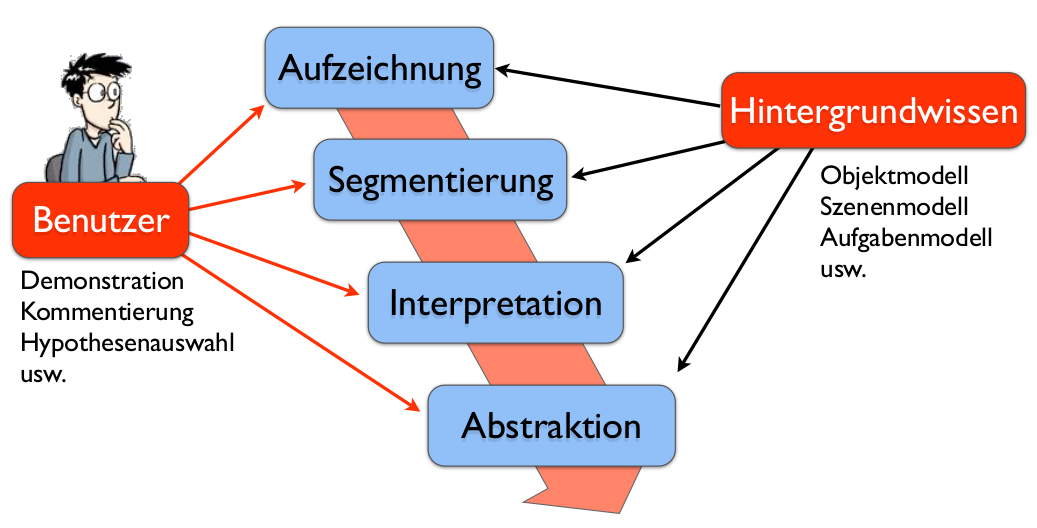
\includegraphics[width=0.6\linewidth]{figures/ch03_verarbeitungsschritte.png}
\caption{Lernsystem: Verarbeitungsschritte}
\label{fig:ch03_verarb}
\end{figure}

Abbildung \ref{fig:ch03_verarb} zeigt die Berarbeitungsschritte eines interaktiven Programmiersystems
%F18 ??
\subsubsection*{Ausführende Manipulatoren}
Ein Manipulator ist ein Roboter, der sich aus einer Steuerung und mechanischen Komponenten (Manipulatorarm) zusammen setzt. Er ist in der Lage, die Position und Orientierung
eines Objektes bezüglich eines Bezugskoordinatensystems zu ändern.
Es sind zwei Arten der Wissensrepräsentation zu unterscheiden, wie in Tabelle \ref{tab:Wissrep} dargestellt.

\begin{table}[hbt]
\centering
\begin{tabular}{|p{8cm}|p{8cm}|}
\hline
Manipulatorabhängige Repräsentation: \newline \textcolor{red}{subsymbolisch} & Manipulatorunabhängige Repräsentation: \newline \textcolor{red}{symbolisch}\\
\hline
Angabe von
\vspace{-4mm}
\begin{itemize}
\setlength\itemsep{0em}
\item Aktionssequenz oder
\item Gelenkwinkel-, Kraft und Momenttrajektorien
\end{itemize}
Nachteile: 
\begin{itemize}
\setlength\itemsep{0em}
\item[-] bei Serviceanwendungen nicht flexibel genug, da invariante Trajektorien keine Veränderung der Lage zu den manipulierten
Objekten in der Umwelt erlauben
\item[-] Variationen in Material, Form und Gewicht beim Manipulationsobjekt können nicht berücksichtigt werden; statische Trajektorien verlieren bei einer Veränderung dieser Werte zur
Programmausführung ihre Gültigkeit
\item[-] unterschiedliche Manipulatoren weisen aufgrund der Kinematik der Manipulatorarme und Endeffektoren verschiedene Konfigurationsräume auf und besitzenverschiedene Sensorausstattung
\item[-] bei expliziter Trajektorienerfassung benötigt man viel Speicher
\item[$\rightarrow$] durch die schwach strukturierte Umwelt und die Forderung von Wiederverwendbarkeit im Dienstleistungsbereich ist die manipulatorabhängige Repräsentation hier nicht sinnvoll
\end{itemize}
 &
 Angabe von Sequenzen von Elementaroperatoren
 \vspace{-4mm}
\begin{itemize}
\setlength\itemsep{0em}
\item Elementaroperatoren sind Regelungen mit Start-, End- und Fehlerkriterien
\item Implementierung der Elementaroperatoren ist manipulatorunabhängig
\item Effekte in der Umwelt sind manipulatorunabhängig, Situation wird nur über lokale Sensorwerte erstellte Umweltinformation beschrieben
\end{itemize}
Bewertung:
\begin{itemize}
\setlength\itemsep{0em}
\item[+] flexible Repräsentation und benutzerfreundliche symbolische Darstellung
\item[+] größere Flexibilität gegenüber Umweltveränderungen und unterschiedlichen Manipulatortypen
\item[+] Elementarfunktionen haben einen hohen Wiederverwendbarkeitswert, so braucht ein Programm nur die Sequenz der Elementarfähigkeiten
enthalten und ihre einzelnen Parameter bestimmen und repräsentieren;  oft weichen in einer
dynamischen Welt die Parameter der Elementarfähigkeiten von denen der Benutzerdemonstration ab, daher werden für variable Parameter Berechnungsfunktionen und
Auswahlbedingungen statt konkreter Werte benutzt
\item[-] Elementarfähigkeiten müssen für jeden Manipulator a-priori erzeugt werden 
\end{itemize}\\
\hline
\end{tabular}
\caption{Arten der Wissenrepräsentation}
\label{tab:Wissrep}
\end{table}

%Tabelle 5.1 Skript!!
\subsection{Wissensrepräsentation: Beispielsysteme}
\subsubsection*{Probabilistisch (Calinon \& Billard)}\footnote{[Calinon07]: What is the teacher’s role in robot programming by demonstration?\\
On learning, representing and generalizing a task in a humanoid robot}
Ziel: Lernen von Skills, z.B. Schachfigur bewegen
\begin{itemize}
\item Aktive, physische Demonstration am Roboter $\rightarrow$ kein Korrespondenzproblem
\item Repräsentation durch Gaussian Mixture Models (GMM) $\rightarrow$ subsymbolisch
\item Direkte Ausführung
\end{itemize}
Hierbei werden folgende Lerndaten benötigt:
\begin{itemize}
\item $(\theta, x, y, h)$: $n$ Demonstrationen mit je $T$ Trajektorienpunkten
\item $\theta$: Gelenkwinkel des Roboters + Zeitstempel
\item $x$: Kartesische Position der Hände + Zeitstempel
\item $y$: Distanzvektor der Hände zur Startposition des Objekts + Zeitstempel
\item $h$: Binärer Zustand des Greifers (offen, geschlossen) + Zeitstempel
\end{itemize}
Das Lernverfahren besteht dann aus folgenden Schritten: 
\begin{itemize}
\item Dimensionsreduktion und zeitliche Angleichung: $(\theta, x, y, h) \rightarrow (\theta^\prime, x^\prime, y^\prime, h^\prime)$
\item Lernen eines GMMs (vgl. Abbildung \ref{fig:ch03_gmm}) für alle Komponenten, z.B. $x^\prime$ (4-dimensional) mit Dichte $p(x^\prime)$:
\begin{align*}
p(x^\prime) = \sum\limits_{i=1}^k p(i)p(x^\prime|i) = \sum\limits_{i=1}^k \pi_i \mathcal{N}(x^\prime; \mu_i, \Sigma_i)
\end{align*} mit $k$ = Anzahl der Normalverteilungen, $\pi$ = Gewichtung, $\mathcal{N}$ = Normalverteilung
\item Bestimmung von $k$: Bayes‘sches Informationskriterium und EM-Algorithmus
\begin{figure}[ht]\centering 
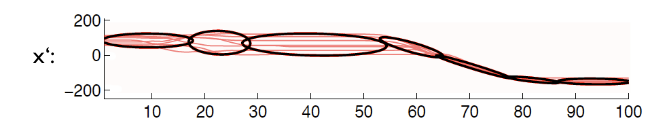
\includegraphics[width=0.6\linewidth]{figures/ch03_gmm.png}
\caption{Gaussian Mixture Model}
\label{fig:ch03_gmm}
\end{figure}
\end{itemize}
\newpage
Die Repräsentation gestaltet sich folgendermaßen:
\begin{itemize}
\item Probabilistische Darstellung der Trajektorien $x^\prime: t \mapsto \mathcal{N}(\mu_{x^\prime}(t), \Sigma_x(t))$
\item Berechnung durch Gaussian Mixture Regression (vgl. Abbildung \ref{fig:ch03_gmr}): Gewichtung der bedingten Wahrscheinlichkeiten $p(x^\prime, i|t)$
\begin{align*}
\mu_{x^\prime}(t) = \sum\limits_{i=1}^k \beta_i(t)\mu_{i, x^\prime|t} \text{ und } \Sigma_{x^\prime}(t) = \sum\limits_{i=1}^k \beta_i(t)^2\Sigma_{i, x^\prime|t}\\
\text{ mit } p(x^\prime,i|t) = \mathcal{N}(\mu_{i, x^\prime|t}, \Sigma_{i, x^\prime|t}) \text{ und } \beta_i(t) = \frac{p(t|i)}{\Sigma{j=1}^k p(t|j)}
\end{align*}
\begin{figure}[ht]\centering 
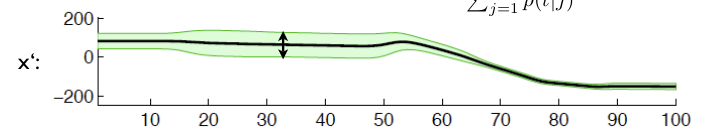
\includegraphics[width=0.6\linewidth]{figures/ch03_gmr.png}
\caption{Gaussian Mixture Regression}
\label{fig:ch03_gmr}
\end{figure}
\end{itemize}
Die Ausführung besteht dann aus folgenden Schritten:
\begin{itemize}
\item Definition eines quadratischen Ähnlichkeitsmaßes: \Gu metric of imitation\Go
\item Gewichtung der Abweichung von den Mittelwerten in $t$, z.B. $\mu_{x^\prime}(t)$
\item Wahl der Gewichtsmatrix: $(\Sigma_{x^\prime}(t))^{-1}$
\item Bestimmung des Nachfolgerzustands $\theta(t+1)$ bzw. der Transition $\theta(t) \rightarrow \theta(t+1)$, die
das Ähnlichkeitsmaß minimiert
\item Jacobi-Matrix zur Kombination von kartesischen und Gelenkwinkeleinschränkungen
\end{itemize}
Eine Bewertung des Verfahrens ist in Tabelle \ref{tab:cabi} dargestellt.
\begin{table}[hbt]
\centering
\begin{tabular}{|p{6.5cm}|p{6.5cm}|}
\hline
Vorteile & Nachteile\\
\hline
\vspace{-5mm}
\begin{itemize}
\setlength\itemsep{0em}
\item[+] schnelles Verfahren, ähnlich Playbackprogrammierung
\item[+] automatische Adaptierung an Änderungen der Objektpositionen
\end{itemize}
 &
 \vspace{-5mm}
\begin{itemize}
\setlength\itemsep{0em}
\item[-] relevante Merkmale manuell definiert, hier z.B. nur Distanz zu Startposition
\item[-] geringe Generalisierung, da keine Vorbedingungen, Ziele, Kollisionen
 keine zielgerichtete Erzeugung von Bewegungen
\item[-] keine Validierung
\end{itemize}\\
\hline
\end{tabular}
\caption{Zusammenfassung: Calinon, Billard}
\label{tab:cabi}
\end{table}\\ 
\subsubsection*{Dynamisch (Pastor \& Schaal)\footnote{[Pastor09]: Learning and generalization of motor skills by learning from demonstration}}
Ziel: Lernen von Skills, z.B. Tennisschwung
\begin{itemize}
\item Aktive, physische Demonstration am Roboter $\rightarrow$ kein Korrespondenzproblem
\item Repräsentation durch Dynamic Movement Primitives (Differentialgleichungen)
\item Direkte Ausführung
\end{itemize}
Die Repräsentation ist wie folgt:
\begin{itemize}
\item Implizite Darstellung durch Menge von Differentialgleichungen:
\begin{align*}
\tau \dot{v} &= K(g-x) -Dv + (g-x_0)f\\
\tau \dot{x} &= v\\
\end{align*}
\item $x$ = Position, $v$ = Geschwindigkeit, $K$ = Federkonstante,
$D$ = Dämpfung, $g$ = Ziel, $x_0$ = Start, $\tau$ = zeitliche Skalierung
\item $f$ = nicht-lineare Funktion, die die Demonstrationsmenge approximiert:
\begin{align*}
f(s) = \frac{\sum_{i=1}^n w_i\psi_i(s)s}{\sum_{i=1}^n \psi_i(s)} \text{ mit } \tau \dot{s} = -\alpha s
\end{align*}
\item Vorteil: Gewichte hängen nicht von $\tau, x_0 $ und $g$ ab
\ita Änderungen von Start, Ziel und der zeitlichen Skalierung möglich
\ita Generalisierung eingeschränkt möglich
\end{itemize}
Das Lernen läuft in folgenden Schritten ab:
\begin{itemize}
\item Berechnung von $v(t), \dot{v}(t)$ für jede Demonstration $x(t)$
\item $s(t)$ wird durch Integration berechnet
\item Der Wert $f(s)$ wird berechnet
\item $\psi_i$ sind nicht normalisierte Normalverteilungen (\Gu Gau{\ss}‘sche Basisfunktionen\Go)
\item Bestimmung der Parameter $w_i$ durch lineare Regression
\end{itemize}
Die Ausführung erfolgt über die Berechnung von $v(t), \dot{v}(t)$ im aktuellen Zustand und Integration.\\
Eine Bewertung des Verfahrens ist in Tabelle \ref{tab:pascha} dargestellt.
\begin{table}[hbt]
\centering
\begin{tabular}{|p{6.5cm}|p{6.5cm}|}
\hline
Vorteile & Nachteile\\
\hline
\vspace{-5mm}
\begin{itemize}
\setlength\itemsep{0em}
\item[+] schnelles Verfahren
\item[+] automatische Adaptierung an Start und Ziel
\item[+] lokale Hindernisvermeidung möglich
\end{itemize}
 &
 \vspace{-5mm}
\begin{itemize}
\setlength\itemsep{0em}
\item[-] relevante Merkmale manuell definiert
\item[-] geringe Generalisierung
\item[-] keine Validierung
\end{itemize}\\
\hline
\end{tabular}
\caption{Zusammenfassung: Pastor, Schaal}
\label{tab:pascha}
\end{table}\\ 
\subsubsection*{Sub-/Symbolisch (IPoR II)}
\textbf{I}nteraktives \textbf{P}r\textbf{o}grammieren von \textbf{R}obotern (IPoR) wurde an der Universität Karlsruhe entwickelt. \\
Problembeschreibung:
\begin{itemize}
\item Robotersystem mit sehr vielen Freiheitsgraden (Kuka LBR / SAH/HIT: 40)
\item  Fingerfertige Manipulation fester Körper („rigid bodies“)
\item Roboterarbeitsraum in realen Situationen stark eingeschränkt (z.B.
Kollisionen)
\item  \Gu Korrespondenzproblem\Go: Mensch und Roboter haben unterschiedliche
Kinematik, d.h. keine direkte Abbildung menschlicher Bewegungen möglich
\end{itemize}
Einsatz von Planungsmethoden:
\begin{itemize}
\item Repräsentation der Manipulationsaufgabe als Bahnplanungsproblem mit Einschränkungen
\item Autonome Planung von Bewegungen, die das Ziel einer Manipulationsaufgabe erfüllen
\item Problem: Manuelle Definition des Planungsproblems ist komplex (z.B. $\leq$ 40 dofs)
\ita Lernen von Planungsproblemen aus der Beobachtung des Menschen
\end{itemize}
Repräsentation als Bahnplanungsproblem mit Einschränkungen:
\begin{itemize}
\item Beschränkung der Bewegung eines Koordinatensystems relativ zu einem zweiten Koordinatensystem (ähnlich \Gu Task Frames\Go) 
\item Drei Typen von Bewegungseinschränkungen:
\begin{itemize}
\item Positionseinschränkungen
\item Orientierungseinschränkungen
\item Richtungseinschränkungen
\end{itemize}
\item Definition: Eine Einschränkung ist ein 5-Tupel $(t, f, M, g, R)$ mit
\begin{itemize}
\item Typ $t$
\item Koordinatensystemen $f, g$
\item homogener Transfromationsmatrix $M$, relativ zu $f$
\item Region $R$
\end{itemize}
%Wiederholungsfolien 35, 36 ausgelassen
\item Wann ist eine Einschränkung erfüllt?
\begin{itemize}
\item Transformation von $M$ definiert in $f$ relativ zu $g$:
\begin{align*}
M^\prime &= ^0H_g^{-1} \cdot ^0 H_f \cdot M\\
M^\prime &= ^g H_f \cdot M
\end{align*}
\item Umwandlung von $M^\prime$ in 3D-Vektor $m^\prime$:\\
$t$ = Position, Richtung: $m^\prime = (x y z)$\\
$t$ = Orientierung: $m^\prime = (r_x r_y r_z )$
\item Bestimmung des nächsten Punkts $n$ in $R$ und der Distanz $d = | m^\prime - n |$
\item Erfüllt, wenn $d < \varepsilon$
\end{itemize}
\item Repräsentation des Planungsproblems als \Gu Strategiegraph\Go :
Tupel $X, C^t_n, C^t_e, C^b_n, C^b_e)$ mit Knoten $X$, zeitliche Einschränkungen der Knoten $C^t_n$ und Kanten $C^t_e$,
Bewegungseinschränkungen der Knoten $C^b_n$ und Kanten $C^b_e$
\end{itemize}
Abbildung \ref{fig:ch03_stratgra} zeigt ein Beispiel eines solchen Graphen.
\begin{figure}[ht]\centering 
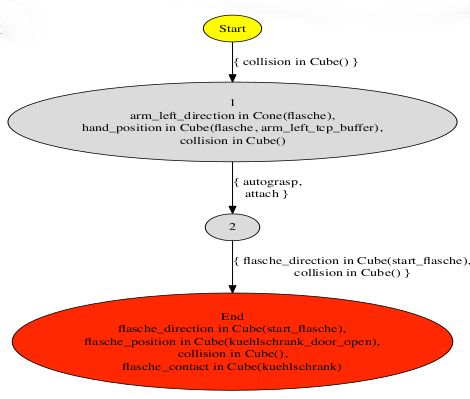
\includegraphics[width=0.6\linewidth]{figures/ch03_strategiegraph.png}
\caption{Beispiel eines Strategiegraphen: \Gu Einschenken\Go $\rightarrow$ Die Ausführungsumgebung bezieht sich auf Unterschiede in Objekten,
Objektposen und Hindernissen (verglichen mit Demonstrationen). Einschränkungen im Strategiegraphen referenzieren Koordinatensysteme. Deren Lage wird automatisch adaptiert. Bei Ausführung unter Verwendung von Bahnplanung repräsentieren die Knoten des Graphen Teilziele der Manipulationsaufgabe, seine Kanten Übergänge zwischen den Teilzielen. Ein Planungsproblems wird für jedes Teilziel gelöst.}
\label{fig:ch03_stratgra}
\end{figure}

\noindent
Im Folgenden soll der PdV-Zyklus (vgl. Abbildung \ref{fig:ch03_zykl}) beispielhaft an IPoR II 
verdeutlicht werden. %Hierzu viele potentiell relevante Bilder auf den Folien 
\paragraph*{Beobachtung} Als Sensorik wird verwendet: Mikrofon, Deckenkameras, Stereokamera mit Pan-Tilt-Unit, Flock-of-Birds, Voodoo, Cybergloves\\
Virtual Technology - Datenhandschuh, Meßprinzip: Dehnmessstreifen, 20 Fingerbeugungs- und Spreizwinkel + 2 Freiheitsgrade im Handgelenk\\
Bestimmung der Position und Orientierung der menschlichen Hände sowie von Objekten: Magnetfeldbasierter Positionstracker, Stereokamera

\paragraph*{Segmentierung}
\begin{itemize}
\item Ziel (mit Interpretationsphase): Repräsentation der demonstrierten Handlung durch Sequenz von zu
erfüllenden Teilzielen (= Topologie des Strategiegraphs)
\item Ansatz: schwellwertbasierte Segmentierung zur Bestimmung von markanten Zeitpunkten der Demonstration
\item Vorteile: einfache Interaktionsmöglichkeit während der Demonstration, einfache Korrektur von Hypothesen
\item Erzeugung eines Segmentierungspunkt, wenn Hand-, Fingergeschwindigkeit gering ist und mindestens ein Finger Objektkontakt % vgl Skript, IPor 1 !!
hat
\end{itemize}

\paragraph*{Interpretation} 
\begin{itemize}
\item Klassifikation der Segmentierungspunkte in 4 Typen auf Basis des Weltzustands an den Intervallgrenzen: 
\begin{itemize}
\item Kein Objekt
\item Objekt aufgenommen
\item Objekt gehalten
\item Objekt losgelassen
\end{itemize}
\item Lernen des Planungsmodells
\begin{itemize}
\item  Topologie des Strategiegraphs: Segmentierung der Bewegungen des linken und rechten Arms, Kombination zu einem Graphen (vgl. \autoref{sg})
\item Erzeugung der Bewegungseinschränkungen: Manuell definierte Koordinatensysteme für alle Objekte: $K = \{ \text{Flaschenöffnung, Becheröffnung,
Rechter Zeigefinger, Welt, ...} \}$; Erzeugung aller möglichen Einschränkungen $(t, f, M, g, R)$ mit $f,g \in K$, Typ $t$ beliebig,
für jeden Knoten und jede Kante $\rightarrow$ Region $R$ muss bestimmt werden (vgl. \autoref{sg1})
\item Beispiel: $f$ = Flaschenöffnung, $g$ = Welt, $t$ = Richtung; $f$ = Flaschenöffnung, $g$ = Becheröffnung, $t$ = Position
\end{itemize}
\begin{figure}[h!]
	\centering
	\begin{subfigure}{.4\textwidth}
		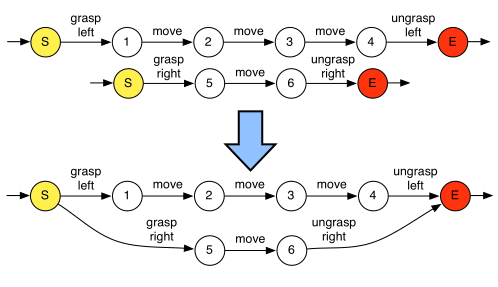
\includegraphics[width=\textwidth]{figures/ch03_stratgraph.png}
		\caption{}
		\label{sg}
	\end{subfigure}
	\begin{subfigure}{.4\textwidth}
		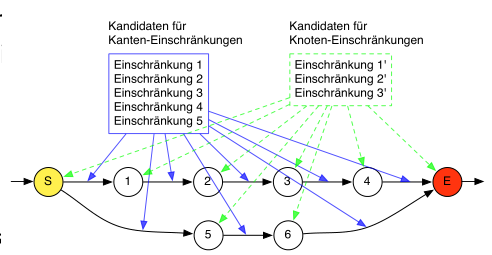
\includegraphics[width=\textwidth]{figures/ch03_stratgraph1.png}
		\caption{}
		\label{sg1}
	\end{subfigure}
	\caption{}
\end{figure}
\item Bestimmung der Region $R$: Für jede Einschränkung $(t, f, M, g, R)$
\begin{itemize}
\item Bestimmung des Werts von $f$ in jedem Punkt $t_i$ des Segments: $g^H_f(t_i) \cdot M$
\item Umwandlung in 3D-Vektor $m^\prime(t_i)$
\item Ergebnis: Menge von 3D-Vektoren
\item Bestimme Region $R$, die alle 3D-Vektoren einschließt
\ita Beispiel: Knoten-Einschränkung ($f$ = Flaschenöffnung, $g$ = Becheröffnung, $t$ = Position)
\end{itemize}
\end{itemize}
\paragraph*{Abstraktion}
Ziel: Anwendbarkeit des Planungsmodells in neuen Situationen auf verschiedenen Robotern
\begin{itemize}
\item Weitere Einschränkungen: Kräfte, Kontakte, Objektbewegung
\item Wesentliche Abstraktion durch Koordinatensysteme und Einschränkungen
\ita Abbildung von objektabhängigen Koordinatensystemen, \\z.B. Flasche.Öffnung $\rightarrow$ Milchpackung.Öffnung
\end{itemize} 

\paragraph*{Ausführung}
\begin{itemize}
\item Gelernte Einschränkungen definieren Suchraum für Roboterbewegungen
\item Einsatz von \textit{Bahnplanung unter Einschränkungen} zur Ausführung von gelernten
Planungsmodellen
\item Einsatz von \textit{Griffplanung} zur Bestimmung qualitativ hochwertiger Griffe
\end{itemize}
Eine Bewertung des Verfahrens ist in Tabelle \ref{tab:ipo} dargestellt.
\begin{table}[hbt]
\centering
\begin{tabular}{|p{6.5cm}|p{6.5cm}|}
\hline
Vorteile & Nachteile\\
\hline
\vspace{-5mm}
\begin{itemize}
\setlength\itemsep{0em}
\item[+] Generalisierung auf Basis von Objekteigenschaften
\item[+] Start- und Zielbeschreibung, Validierbarkeit
\item[+] Hindernisvermeidung und Berücksichtigung von Einschränkungen
\item[+] mehrere Lösungen und beliebige Optimalitätskriterien
\end{itemize}
 &
 \vspace{-5mm}
\begin{itemize}
\setlength\itemsep{0em}
\item[-] hoher Aufwand (Planungszeit, Simulationszeit)
\item[-] 3d-Modelle der Objekte, menschlichen Hand notwendig
\item[-] automatische Segmentierung bei dynamischen Bewegungen schwierig
\end{itemize}\\
\hline
\end{tabular}
\caption{Zusammenfassung: IPOR II}
\label{tab:ipo}
\end{table}\\ 
%Nächste VL:
%• Bahnplanung
%• Grifftaxonomie
%• Griffplanung